\section{Аналитический раздел}
\subsection{Постановка задачи}
В соответствии с заданием на курсовую работу по курсу <<Операционные системы>> необходимо разработать программное обеспечение,
позволяющее использовать геймпада в качестве компьютерной мыши.\par
Для реализации поставленной задачи требуется:
\begin{itemize}
	\item проанализировать существующие драйвера геймпадов;
	\item разработать загружаемый модуль, позволяющий использовать функционал компьютерной мыши
	при помощи геймпада;
	\item реализовать программное обеспечение;
	\item выполнить тестирование разработанного модуля.
\end{itemize}
Программное обеспечение должно позволять использовать клавиши геймпада, как аналоги левой и правой клавиш мыши, перемещать курсор при помощи левого стика, пролистывать страницы при помощи правого.\par

\subsection{Загружаемый модуль ядра}
Несмотря на то, что ядро Linux является монолитным, оно позволяет
выполнять вставку и удаление кода ядра в процессе работы. Для этого нужны загружаемые модули ядра.\par
Модуль по своей сути примерно то же, что и обычная программа. Модуль
так же имеет точку входа и выхода. Но
модули имеют непосредственный доступ к структурам и функциям ядра. Для
программ в пространстве пользователя этот доступ ограничен\cite{soloviev}.\par
%Соловьев А. Разработка модулей ядра ОС Linux Kernel newbie's manual.
Использование загружаемых модулей значительно упрощает изменение
функциональности ядра и не требует ни полной перекомпиляции, ни перезагрузок.Также преимущество загружаемых модулей заключается в возможности сократить расход памяти для ядра, загружая только
необходимые модули.\par
Загрузка модуля осуществляется с помощью команд \textit{insmod} или
\textit{modprobe}. Отличие заключается в том, что \textit{modprobe} разрешает зависимости
модулей. При загрузке вызывается функция входа, определенная в модуле.\par
Для указания ее назначения используется макрос \textit{module\_init}. При корректной
загрузке функция входа возвращает 0. В ином случае, модуль не будет
загружен.\par
Для просмотра списка загруженных модулей и информации об
отдельном модуле используются команды \textit{lsmod} и \textit{modinfo} соответственно.
Команда \textit{rmmod} осуществляет выгрузку модуля, при которой
вызывается функция выхода. Для нее используется макрос \textit{module\_exit}.

\subsection{USB шина}
Universal Serial Bus (USB, Универсальная Последовательная Шина) является соединением
между компьютером и несколькими периферийными устройствами. Первоначально она была
создана для замены широкого круга медленных и различных шин, параллельной,
последовательной и клавиатурного соединений, на один тип шины, чтобы к ней могли
подключаться все устройства\cite{Corbet}.\par
%Corbet J., Rubini A., Kroah-Hartman G. Драйверы устройств Linux, Третья редакиця.

USB Core — это подсистема ядра Linux, созданная для поддержки USB-устройств и контроллеров шины USB. Ядро USB предоставляет интерфейс для драйверов USB, используемый для доступа и
управления USB оборудованием, без необходимости беспокоится о различных типах
аппаратных контроллеров USB, которые присутствуют в системе.\par

Шина USB обеспечивает обмен данными между хост-компьютером и множеством периферийных устройств. USB является единой централизованной аппаратно-программной системой массового обслуживания устройств и прикладных программных процессов. Связь этих процессов со всеми устройствами обеспечивает хост-контроллер с многоуровневой программной поддержкой.\par

%Источник: http://perscom.ru/usb
\subsection{USB драйвер}
Ядро Linux поддерживает два основных типа драйверов USB: драйверы на хост-системе и
драйверы на устройстве. USB драйверы для хост-системы управляют USB-устройствами,
которые к ней подключены, с точки зрения хоста (обычно хостом USB является персональный
компьютер.) USB-драйверы в устройстве контролируют, как одно устройство видит хост-компьютер в качестве устройства USB.\par
Драйверы основного ядра обращаются к прикладным
интерфейсам USB ядра. В тоже время принято выделять два основных
публичных прикладных интерфейса: один --- реализует взаимодействие с
драйверами общего назначения (символьное устройство), другой ---
взаимодействие с драйверами, являющимися частью ядра (драйвер хаба).
Второй тип драйверов участвует в управлении USB шиной.\par
На Рисунке \ref{USB-device} 
представлена, как USB-устройства состоят из конфигураций, интерфейсов и оконечных точек и как USB
драйверы связаны с интерфейсами USB, а не всего устройства USB.

\begin{figure}[h!]
	\centering
	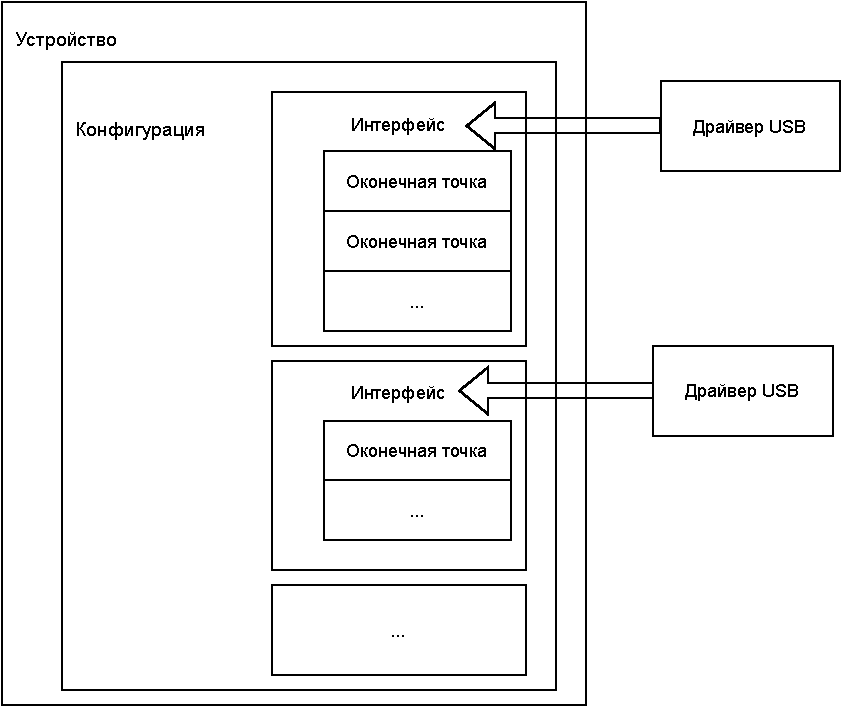
\includegraphics[scale=0.9]{img/Usb-device.pdf}
	\caption{Схема взаимодействия устройства и драйвера}
	\label{USB-device}
\end{figure}\par

\subsection{Оконечная точка}
Самый основной формой USB взаимодействия является то, что называется endpoint
(оконечная точка). Оконечная точка USB может переносить данные только в одном
направлении, либо со стороны хост-компьютера на устройство (называемая оконечной точкой
OUT) или от устройства на хост-компьютер (называемая оконечной точкой IN). Оконечные
точки можно рассматривать как однонаправленные трубы.\par
Драйвер геймпада имеет только 1 конечную точку типа INTERRUPT(прерывание). Для
конечных точек данного типа характерна передача небольшого объема данных
с фиксированной частотой.\par Этот тип оконечных точек являются основным транспортным методом не только для
геймпадов, но и для USB клавиатур и мышей.
Передачи данного типа имеют зарезервированную пропускную способность. \par
Помимо типа INTERRUPT есть ещё 3:  CONTROL (Управление), BULK (Поток),  ISOCHRONOUS (Изохронная).\par

Управляющие оконечные точки используются для обеспечения доступа к различным
частям устройства USB. Они широко используются для настройки устройства, получения
информации об устройстве, посылке команд в устройство, или получения статусных
сообщений устройства. Эти оконечные точки, как правило, малы по размеру.\par

Поточные оконечные точки передают большие объёмы данных. Они являются обычными для устройств, которые должны
передавать любые данные, которые должны пройти через шину, без потери данных.
Эти оконечные точки общеприняты на принтерах,
устройствах хранения и сетевых устройствах.\par

Изохронные оконечные точки также передают большие объёмы данных, но этим данным
не всегда гарантирована доставка. Эти оконечные точки используются в устройствах,
которые могут обрабатывать потери данных, и больше полагаются на сохранение
постоянного потока поступающих данных. При сборе данных в реальном времени, таком,
как аудио- и видео-устройства, почти всегда используются такие оконечные точки.
\par

Управляющие и поточные оконечные точки используются для асинхронной передачи
данных, когда драйвер решает их использовать. Оконечные точки прерывания и изохронные
точки являются периодическими. Это означает, что эти оконечные точки созданы для
передачи данных непрерывно за фиксированное время, что приводит к тому, что их пропускная
способность защищена ядром USB

\subsection{Транзакции и пакеты}
Протокол шины USB обеспечивает обмен данными между хостом и устройством. На протокольном уровне решаются такие задачи, как обеспечение достоверности и надежности передачи, управление потоком. Весь трафик на шине USB передается посредством транзакций, в каждой транзакции возможен обмен только между хостом и адресуемым устройством (его конечной точкой). Все транзакции (обмены) с устройствами USB состоят из двух-трех пакетов, типовые последовательности пакетов в транзакциях приведены на Рисунке \ref{packets}.\par

\begin{figure}[h!]
	\centering
	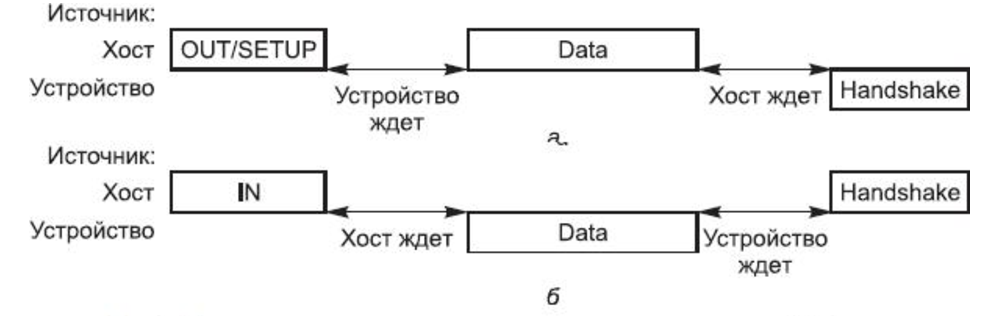
\includegraphics[scale=0.9]{img/packets.pdf}
	\caption{Последовательность пакетов в транзакциях на шине USB:\\
	a - вывод; б - ввод данных}
	\label{packets}
\end{figure}\par

 Каждая транзакция планируется и начинается по инициативе хост-контроллера, который посылает пакет-маркер транзакции (token packet). Маркер транзакции описывает тип и направление передачи, адрес выбранного устройства USB и номер конечной точки. Адресуемое маркером устройство распознает свой адрес и готовится к обмену. Источник данных, определенный маркером, передает пакет данных. На этом этапе транзакции, относящиеся к изохронным передачам, завершаются — здесь нет подтверждения приема пакетов. Для остальных типов передач работает механизм подтверждения, обеспечивающий гарантированную доставку данных\cite{usb}. Типы пакетов приведены ниже на Рисунке \ref{packets-types}.
\begin{figure}[h!]
	\centering
	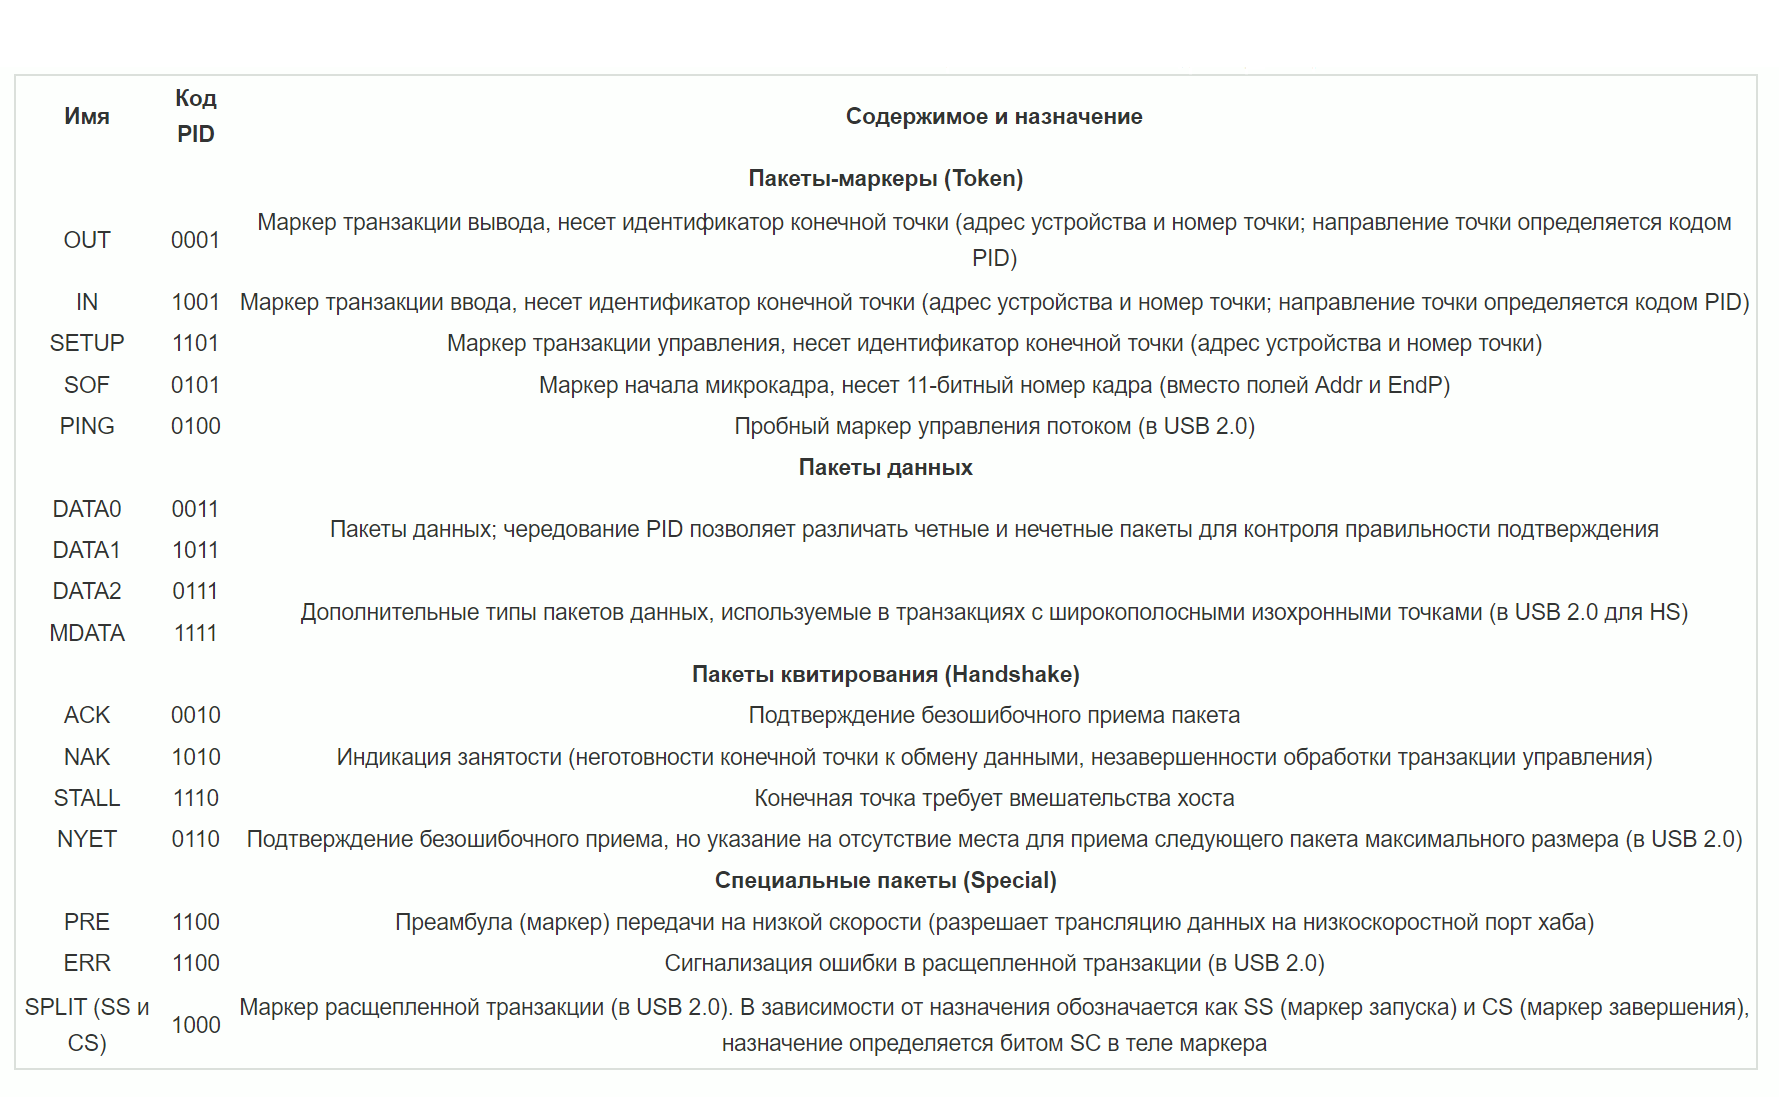
\includegraphics[scale=0.46]{img/packets-types.png}
	\caption{Типы пакетов и их идентификаторы PID}
	\label{packets-types}
\end{figure}\par

\subsection{Блоки запроса USB}
urb используется для передачи или приёма данных в или из заданной оконечной точки USB
на заданное USB устройство в асинхронном режиме. Каждая оконечная точка в
устройстве может обрабатывать очередь urb-ов, так что перед тем, как очередь опустеет, к
одной оконечной точке может быть отправлено множество urb-ов. Типичный жизненный цикл
urb выглядит следующим образом:
\begin{itemize}
	\item создание драйвером USB;
	\item назначение в определённую оконечную точку заданного USB устройства;
	\item передача драйвером USB устройства в USB ядро;
	\item передача USB ядром в заданный драйвер контроллера USB узла для указанного
	устройства;
	\item обработка драйвером контроллера USB узла, который выполняет передачю по USB в
	устройство;
	\item после завершения работы с urb драйвер контроллера USB узла уведомляет драйвер USB
	устройства.
\end{itemize}

\subsection{Выводы}
В результате проведенного анализа были рассмотрены принцип работы и способы реализации загружаемого модуля ядра,
позволяющего использовать геймпад как компьютерную мышь. В качестве реализации был выбран USB-драйвер геймпада.

\pagebreak

